\documentclass[12pt, a4paper]{report}
\usepackage[italian]{babel}
\usepackage[T1]{fontenc}
\usepackage[sfdefault]{noto}
\usepackage{graphicx}
\usepackage{multirow}
\usepackage{enumitem}
\usepackage{hyperref}
\hypersetup{pdfborder = 0 0 0 }
\usepackage{wrapfig}
\usepackage{color}
\usepackage{tabularx}
\usepackage{makecell}
\linespread{1.3}
\textwidth=450pt\oddsidemargin=0pt
\begin{document}
\begin{titlepage}
\vspace{15mm}
\begin{center}
  
\includegraphics{Images/uniboLogo}
\end{center}
\begin{center}
{\normalsize{\bf Corso di Laurea Magistrale in Informatica}}\\
\vspace{5mm}
{\normalsize{\bf Anno Accademico 2018/2019}}\\
\vspace{20mm}
{\Large{\bf Software Architecture}}\\
\vspace{10mm}
{\Huge{\bf Kubernetes}}\\
\vspace{25mm}
\end{center}
\begin{flushright}
{\large{Matteo Marchesini\\0000856336\\matteo.marchesini12@studio.unibo.it}}
\end{flushright}
\end{titlepage}
\tableofcontents
\chapter{Descrizione del sistema}
\begin{center}
  
\includegraphics[scale = 0.9]{Images/kubernetesLogo}
\end{center}
Kubernetes è un sistema open source per la gestione di applicazioni containerizzate tra più host; fornisce un meccanismo per il deployment, la manutenzione e lo scaling di applicazioni. È stato inizialmente sviluppato dal team di Google, per poi passare nel 2015 sotto il controllo del \textit{Cloud Native Computing Foundation (CNCF)}, che attualmente lo supporta.\\ Al giorno d'oggi è uno dei sistemi di orchestrazione per applicazioni conteinerizzate più utilizzato in assoluto, con una vastità di utenti, partners e una comunità di development attiva. Non a caso tre dei quattro maggior providers di servizi Cloud - Microsoft, IBM e Google - offrono piattaforme di Container as a Service (CaaS) basate su Kubernetes. I servizi che Kubernetes mette a disposizione sono molteplici: fornisce un ambiente la gestione di container, microservizi e piattaforme cloud. Inoltre organizza l'infrastruttura di rete e di archiviazione per conto dell'utente.\\
In generale un sistema distribuito necessita di più componenti per il corretto funzionamento, alcune open source e altre commerciali; invece Kubernetes da solo fornisce uno scenario in cui le componenti lavorano insieme, andando così a formare un unico componente combinando la semplicità del Platform as a Service (PaaS) con la flessibilità dell'Infrastructure as a Service (IaaS).\\
L'orchestrazione di container ha avuto un profondo impatto in ogni aspetto del software development e deployment moderno; in particolare ha influenzato l'architettura del Platform as a Service, fornendo un aperto ed efficiente modello per il packaging, deployment, isolamento, scaling e rolling upgrade. Kubernetes svolgerà un ruolo cruciale nell'utilizzo di container da parte di imprese e start-up emergenti.
\\L'oggetto di questo report è di studiare tutto ciò che riguarda e circonda l'architettura di Kubernetes.
\chapter{Contesto}
\section{Scopo del sistema}
In questo capitolo verrà discusso lo scopo di Kubernetes e la sua interazione con le entità esterne, nonchè i principali casi d'uso. \\
Kubernetes, come introdotto nel Capitolo 1, è un sistema di orchestrazione di container e per questo motivo si occupa principalmente di \textbf{deployment}, \textbf{scaling} e \textbf{management} di applicazioni containerizzate. Di seguito viene definito ognuno di questi tasks:
\begin{itemize}
\item \textbf{Deployment}: gestisce la distribuzione di applicazioni assegnando ai nodi del cluster ciascuna istanza dell'applicazione. Il deployment in Kubernetes può essere eseguito in una varietà di ambienti con pattern differenti, ed esistono appunto diversi modelli, quali:
\begin{itemize}
  \item Container as a Service (CaaS);
  \item Public Cloud - Infrastructure as a Service (IaaS);
  \item Utilizzo on-premises all'interno di data center;
  \item Deployment ibrido
\end{itemize}
\item \textbf{Scaling}: permette di ridimensionare l'applicazione a seconda delle esigenze dell'utente, andando a modificare le dimensioni del cluster e il numero di repliche dei pod. Un \textbf{pod} è il più piccolo oggetto deployabile nel modello a oggetti di Kubernetes e può incapsulare un singolo container o più container che necessitano di lavorare insieme.
\item \textbf{Management}: fornisce un'interfaccia per la gestione dei cluster e delle applicazioni containerizzate. Un cluster di Kubernetes viene ospitato e gestito da un venditore commerciale, quali ad esempio Google Container Engine (GKE), Amazon EC2 Container Service e Azure Container Service di Microsoft, che offrono servizi di CaaS nel cloud pubblico. Molti utenti hanno iniziato ad usare Kubernetes attraverso Google Container Engine, essendo uno dei primi servizi di gestione di Kubernetes nel mercato.
\end{itemize}
\section{Entità esterne}
Nella figura seguente è espresso il \textit{system context diagram} di Kubernetes, che definisce le relazioni tra esso e le entità esterne.
\begin{center}
  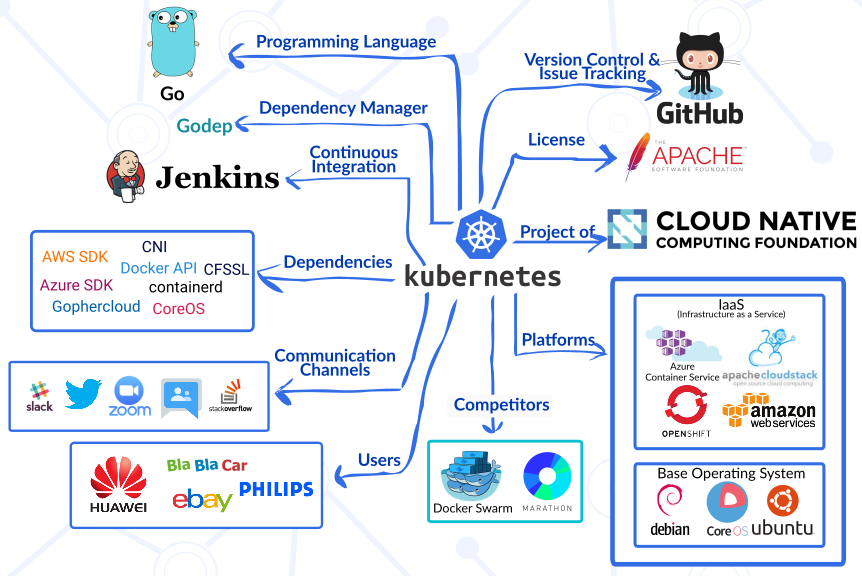
\includegraphics[scale = 0.6]{Images/ContextModelDiagram}
\end{center}
Le entità di maggior rilievo all'interno del diagramma e che verranno analizzate in seguito sono gli stakeholders, il development, le piattaforme e i concorrenti.
\subsection{Stakeholders}
Per poter comprendere al meglio il concetto di stakeholder all'interno di un progetto così grande come quello di Kubernetes, è necessario introdurre il \textbf{Cloud Native Computing Foundation} (CNCF).\\
CNCF è nato nel 2015 da un accordo tra Google e la Linux Foundation con l'annuncio di Kubernetes 1.0, considerato il progetto principale. Da li in poi molte industrie del cloud computing si sono unite a CNCF per incubare, sviluppare e mantenere un ecosistema di progetti cloud sotto una visione comune e condivisa. I membri di CNCF sono divisi per categorie, quali Platinum, Gold, Silver, End-User, accademici e no-profit. Tra i membri Platinum abbiamo Google, Docker, IBM, Cisco e Oracle.\\
Oltre all'organizzazione CNCF, Kubernetes attrae migliaia di contributori che coordinano i loro sforzi attraverso piattaforme online, quali GitHub, Slack e StackOverflow (fornitori). Gli Special Interest Groups (SIG) si occupano dello sviluppo di Kubernetes, in particolare dell'architettura, del product management e del testing, nonchè di implementazione specifiche per fornitori di servizi come AWS e Azure.
\subsubsection{Griglia Power/Interest}
Nella seguente immagine è raffigurata la griglia o matrice \textit{power/interest} che divide gli stakeholders in quattro categorie:
\begin{itemize}
  \item \textbf{Alta potenza e alto interesse}: la massima potenza suoi progetti di Kubernetes la detiene il consiglio d'amministrazione di CNCF che ne gestisce il budget, seguito poi da CNCF TOC (Technical Oversight Committee), che ha il compito di aggiungere e rimuovere progetti come Kubernetes. Inoltre anche l'architettura SIG è fondamentale in quanto decide il futuro del progetto.
  \item \textbf{Alta potenza e basso interesse}: il CNCF Marketing Committee, derivato dal consiglio di amministrazione di CNCF, cura il brand del progetto e altre attività legate al business.
  \item \textbf{Bassa potenza e alto interesse}: rispetto agli stakeholder con grande potere su Kubernetes, il CNCF end user TAB, lo staff di provider di piattaforme/servizi, Test SIG e la comunità di sviluppatori generali di Kubernetes dipendono dal continuo sviluppo del progetto, e questo comporta un alto interesse.
  \item \textbf{Bassa potenza e basso interesse}: le piattaforme di coordinamento, quali GitHub, hanno scarso potere ed interesse per il progetto, in quanto altre piattaforme potrebbero avere uno scopo simile se non fossero prese in considerazione.
\end{itemize}
\begin{center}
  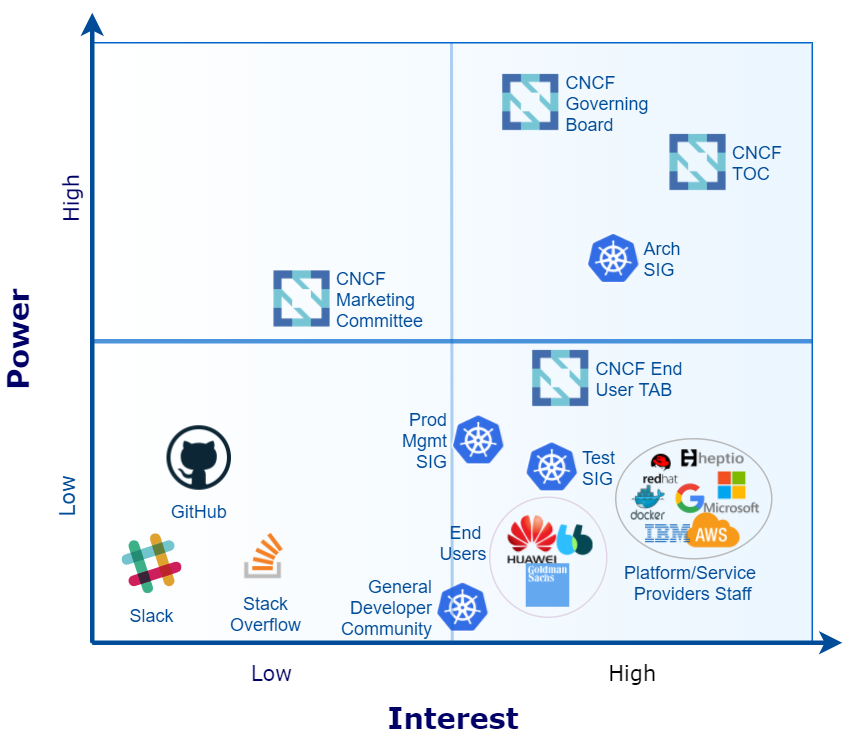
\includegraphics[scale = 0.45]{Images/power-interest}
\end{center}
\subsection{Development}
Il principale linguaggio con cui Kubernetes è sviluppato è \textbf{Go}, un linguaggio open-source progettato da tre ingegneri di Google, ma nonostante ciò possiede dipendenze da varie librerie esterne, quali Amazon Web Services SDK (AWS), Docker API, Azure SDK,  Container Network Interface (CNI), e Gophercloud. Inoltre Kubernetes si affida a Jenkins per la Continuous Integration.
\subsection{Piattaforme}
Kubernetes essendo una piattaforma cloud è compatibile con diverci providers a seconda delle necessità e dell'utilizzo. Di seguito sono riportate alcune soluzioni differenti a seconda del pattern di utilizzo.
\subsubsection{Container Management, soluzioni in locale e PaaS}
\begin{table}[ht]
  \small
  \begin{center}
  \begin{tabularx}{\textwidth}{|lr|}
    \hline
    \textbf{Prodotto} (compagnia) & \textbf{Categoria}\\
    \hline
    \textbf{AppsCode} (AppsCode)&Hosted, PaaS\\
    \multicolumn{2}{|X|}{\textit{È una piattaforma integrata per il deployment, testing e coding di app containerizzate. Permette il deployment su Google Cloud Platform e AWS.}}\\
    \hline
    \textbf{Cloud Container Engine} (Huawei)&CaaS\\
    \multicolumn{2}{|X|}{\textit{Servizio di containerizzazione scalabile ad alte prestazioni basato su Kubernetes}}\\
    \hline
    \textbf{Giant Swarm} (Giant Swarm)&Hosted, on-premises\\
    \multicolumn{2}{|X|}{\textit{Una soluzione creare, distribuire e gestire servizi containerizzati con Kubernetes come componente principale}}\\
    \hline
    \textbf{Google Container Engine} (Google)&CaaS\\
    \multicolumn{2}{|X|}{\textit{Google Container Engine è un sistema di gestione e orchestrazione dei cluster che consente agli utenti di eseguire container sulla piattaforma Cloud di Google}}\\
    \hline
    \textbf{OpenShift Container Platform} (RedHat)&PaaS, on-premises\\
    \multicolumn{2}{|X|}{\textit{Una piattaforma di applicazioni per container che può estendersi su più infrastrutture. È costruito usando la tecnologia Docker e Kubernetes.}}\\
    \hline
  \end{tabularx}
  \end{center}
\end{table}

\begin{table}[ht]
\small
\centering
\begin{tabularx}{\textwidth}{|lr|}
\hline
\textbf{OpenShift Online} (RedHat)&Hosted\\
\multicolumn{2}{|X|}{\textit{Versione hosted di OpenShift. Il funzionamento è il medesimo a quello di OpenShift Container Platform}}\\
\hline
\textbf{Platform9 Managed Kubernetes for Docker} (Platform9)&Hosted, on-premises\\
\multicolumn{2}{|X|}{\textit{I clienti possono utilizzare il singolo pannello di Platform9 per 􏰅orchestrare e gestire i container insieme alle macchine virtuali. In altre parole, è possibile orchestrare le VM's usando OpenStack e/o Kubernetes}}\\
\hline
\end{tabularx}
\end{table}

\subsubsection{Tools per deployment e controllo di clusters Kubernetes}
\begin{table}[ht]
\small
\centering
\begin{tabularx}{\textwidth}{|lr|}
\hline
\textbf{Prodotto} (compagnia) & \textbf{Categoria}\\
\hline
\textbf{AppFormix} (AppFormix)&Monitoring\\
\multicolumn{2}{|X|}{\textit{Fornisce metriche e analisi per i container organizzati con l'architettura di Kubernetes. Gli utenti possono vedere analisi e gestire avvisi, o regole di orchestrazione per singoli pods o container. La dashboard può essere ulteriormente personalizzata e mappata nei propri progetti}}\\
\hline
\textbf{Bootkube} (CoreOS)&Deploy\\
\multicolumn{2}{|X|}{\textit{Uno strumento di supporto per l'avvio di cluster Kubernetes autogestiti.}}\\
\hline
\textbf{ElasticBox ElasticKube} (CenturyLink)&Deploy\\
\multicolumn{2}{|X|}{\textit{Un servizio per connettere pipeline di CI/CD, per la configurazione di tools di management e per il deployment di applicazioni cloud. Inoltre include ElasticKube, una piattaforma open source per Kubernetes che promuove il self-service per le applicazioni containerizzate.}}\\
\hline
\textbf{Kubernetes Dashboard} (Cloud Native Computing Foundation)&Monitor\\
\multicolumn{2}{|X|}{\textit{Fornisce un'interfaccia utente basata sul Web per cluster Kubernetes. Consente agli utenti di gestire le applicazioni in esecuzione nel cluster nonché di gestire il cluster stesso.}}\\
\hline
\textbf{Minikube} (Cloud Native Computing Foundation)&Deploy\\
\multicolumn{2}{|X|}{\textit{Minikube è un tool che semplifica l'esecuzione in locale di Kubernetes. Minikube esegue un cluster Kubernetes a nodo singolo all'interno di una VM sul laptop. Orientato agli utenti che desiderano provare Kubernetes o svilupparlo giorno per giorno.}}\\
\hline
\end{tabularx}
\end{table}
\subsection{Concorrenti}
\chapter{Drivers architetturali}
\chapter{Struttura}
\chapter{Funzioni}
\chapter{Comportamento}
\chapter{Razionale}
\chapter{Aspetti analitici}
\chapter{Stili architetturali simili o derivati}
\chapter{Referenze}
\end{document}
